%!TEX root = ../main.tex

\yyyymmdddate
\renewcommand{\dateseparator}{-}
\newcommand{\tabitem}{~~\llap{\textbullet}~~}

\renewcommand*\ttdefault{txtt}
\newcommand{\ms}[1]{\mbox{\tt #1}\xspace}
\newcommand{\seq}{{\bf s}\xspace}
\newcommand{\strS}{{\mathcal S}\xspace}
\newcommand{\strOff}{\ensuremath{{\mathcal S}_{\text{off}}}\xspace}
\newcommand{\strOn}{\ensuremath{{\mathcal S}_{\text{on}}}\xspace}
\newcommand{\strConst}[1]{\ensuremath{{\mathcal C}_{\text{#1}}}\xspace}
\newcommand{\tree}{{\mathcal T}\xspace}
\newcommand{\treeFor}[1]{\ensuremath{{\mathcal T}_{\text #1}}}
\newcommand{\fnaRetrievalTime}{\formatdate{25}{11}{2014} at \formattime{9}{14}{0}}
\newcommand{\textdown}[2]{\ensuremath{{\text{#1}}_{\text{#2}}}}
\newcommand{\treePos}[2]{\textdown{\ms{#1}}{#2}}
\newcommand{\treeIdx}[3]{\treePos{#1}{#2}\ensuremath{(#3)}}

\newcommand{\rfinder}{\ms{Ribofinder}}
\newcommand{\infernal}{\ms{Infernal}}
\newcommand{\tthp}{\ms{TransTermHP}}
\newcommand{\rshapes}{\ms{RNAshapes}}
\newcommand{\rfold}{\ms{RNAfold}}
\newcommand{\foldalign}{\ms{FoldAlign}}

\chapter{Ribofinder} % Main chapter title

\label{Ribofinder} % For referencing the chapter elsewhere

\lhead{Chapter X. \emph{Ribofinder: A Riboswitch Detection Pipeline}} % This is for the header on each page

Riboswitches are regulatory mRNA elements that modulate gene expression via structural changes induced by the direct sensing of a small-molecule metabolite. Most often found in bacteria, \rbs regulate diverse pathways including the metabolism and transport of purines, methionine, and thiamin amongst others. The structure of a \rb includes an aptamer domain---involved in the direct sensing of the small-molecule---and an expression platform whose structure changes upon the aptamer binding the metabolite. Because of the discriminatory nature of metabolite sensing, groups have had great success in finding representative examples of aptamers across a diverse collection of bacterial species; RFam 12.0 currently contains 26 different families of aptamers involved in different metabolic pathways. Whereas there exists strong sequence and structural similarity within the aptamer of a \rb family, the expression platform is highly variable, and thus challenging to capture using traditional SCFG-based approaches. For this reason databases such as RFam only contain the aptamer portion of the \rb, and there exists no database providing sequences including expression platforms, necessary for capturing the `on' and `off' conformations of this regulatory element. We have developed a new pipeline---called \rfinder---which can detect putative \rbs including their expression platforms and likely conformational structures across a wide collection of genomic sequences.

\section{Pipeline} \label{sec:pipeline}

At the time of our retrieval (\fnaRetrievalTime), the RefSeq database hosted by NCBI comprised 5,121 complete bacterial genomes with corresponding genomic annotations. In order to both detect putative full \rbs across this collection of data as well as filter the candidates down to a number tractable for experimental validation, we developed a novel pipeline which takes a three-tiered approach to candidate selection. Our approach is to \begin{inparaenum}[\itshape a\upshape)]
\item identify a pool of candidate \rbs across genomic data;
\item perform a coarse-grained filtering of the candidate pool based on structural characteristics; and finally
\item fine-grained curation of the candidates based on a collection of measures and pairwise similarity.
\end{inparaenum}

In the following discussion, we describe the application of \rfinder to identify unannotated G-box purine \rbs; guanine-sensing cis-regulatory elements which modulate the expression of genes involved in purine biosynthesis.

\subsection{Candidate Selection} \label{sub:candidates}

The RefSeq data we used for analysis contains 5,121 annotated bacterial genomes across 2,732 different organisms, totaling over $9.5 * 10^9$ bases. We used the program \infernal to determine the coordinates of putative aptamer structures within the RefSeq genomes, and \tthp to locate candidate rho-independent transcription terminators.

\subsubsection{Detecting Aptamers with \infernal} \label{ssub:infernal}

\infernal uses a stochastic context-free grammar (SCFG) with a user-provided multiple sequence alignment (MSA) to efficiently scan genomic data for RNA homologs, taking into consideration both sequence and structural conservation. Using the purine aptamer MSA from RFam 12.0 (RF00167), \infernal (v1.1.1, default options) detects 1,537 significant hits having E-value $<= 0.01$. Because \infernal leverages the concept of a `local end'---a large insertion or deletion in the alignment at reduced cost---it is possible for the software to return a significant hit whose aligned structure does not have the canonical three-way junction observed in all purine \rbs. \rfinder prunes these truncated \infernal hits by converting the alignment structure into a parse tree, and only permitting trees of sufficient complexity to contain a multiloop (described further in \ref{sub:shapes}). The pyrimidine residue abutted next to the P1 stem in the J3-1 junction differentiates between guanine and adenine-sensing \rbs by binding the complimentary purine ligand; for our interest in G-box \rbs exclusively we require the presence of a cytosine at this residue. In total, using \infernal with these additional filters yields 1,280 G-box aptamers across 555 unique organisms (note: here and elsewhere I define a `unique organism' as having a unique taxonomy ID).

\subsubsection{Detecting Expression Platforms with \tthp} \label{ssub:tthp}

\tthp detects rho-independent terminators in bacterial genomes in a context-sensitive fashion by leveraging the protein annotations available in PTT data. These terminator sequences canonically have a stable hairpin loop structure immediately preceding a run of $5+$ uracil residues, the combination of which causes the ribosomal machinery to stall and dissociate from the transcript. \tthp performs a genomic scan to determine candidate loci with this motif, and returns scored hits. The scoring system considers both structural homology and the genomic contextual information available in the PTT file. Across our collection of bacterial genomes acquired from NCBI RefSeq data, \tthp identified 2,752,469 rho-independent terminators using the default filters.

Due to the spatially-mediated structural regulation of purine \rbs, whereby ligand interaction with the aptamer domain induces local structural rearrangement in the expression platform, we paired aptamers with corresponding terminators by minimizing the genomic distance, with an upper bound of 200 nucleotides between the end of the aptamer domain and start of the terminator. This approach yields 577 candidate \rbs, 81 of which have multiple rho-independent terminators within range of a putative aptamer produced by \infernal. For these, we simply pair the closest \tthp hit with the aptamer domain.

\begin{figure}[!ht]
  \centering
    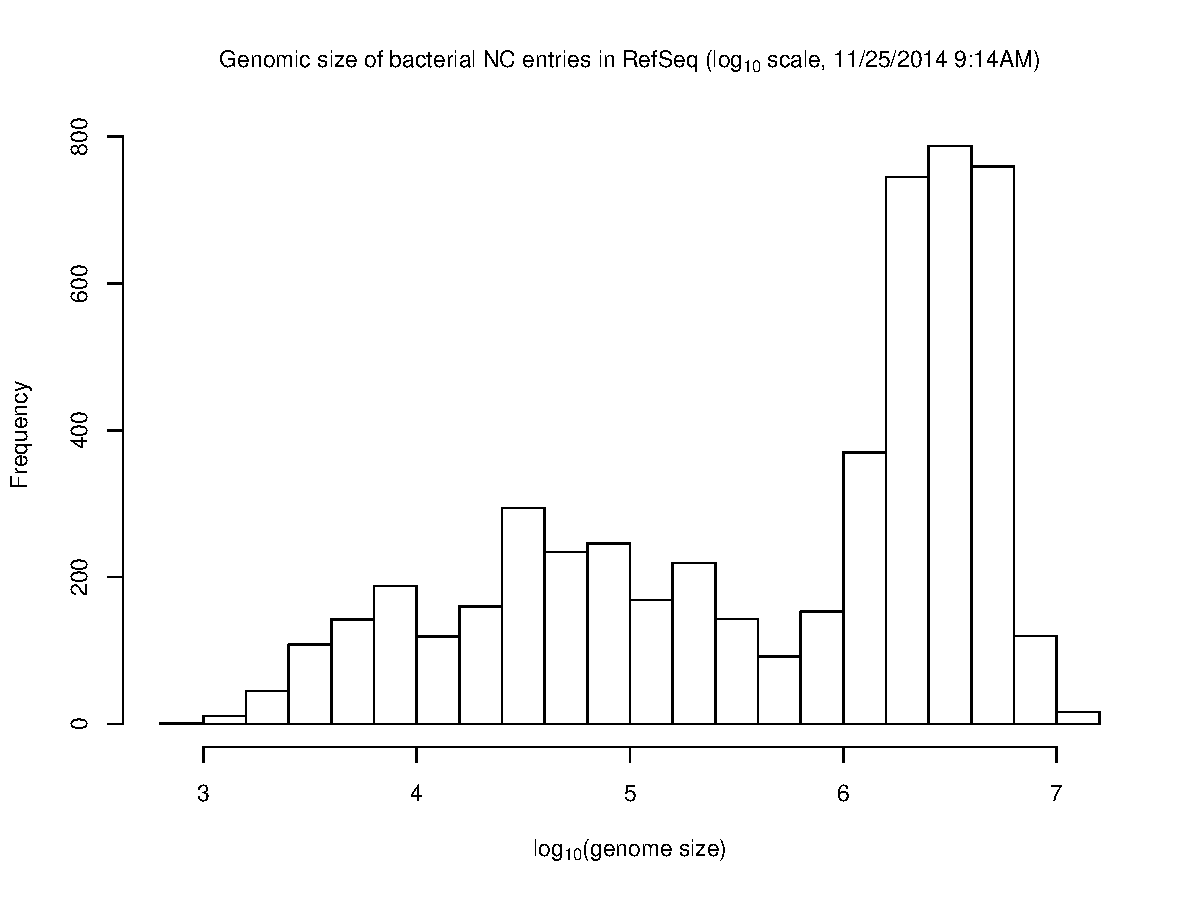
\includegraphics[width=.75\textwidth]{Figures/Ribofinder/refseq_genome_sizes.pdf}
  \caption{Histogram displaying the distribution of genome sizes across the RefSeq data analyzed, comprising 5,172 bacterial genomes. Genome size is shown using a $\log_{10}$ scale.}
  \label{fig:genome_sizes}
\end{figure}

\subsection{Notation for Representing Abstract RNA Shapes} \label{sub:shapes}

Given an RNA sequence $\seq = a_1, a_2, \cdots, a_n$, where positions $a_i$ are drawn from the collection of single-letter nucleotide codes, i.e. $\{\text{A},\text{U},\text{G},\text{C}\}$, it is possible to describe a corresponding secondary structure $\strS$ compatible with \seq using the dot-bracket notation. In this notation, each nucleotide $a_i$ has a corresponding state $s_i$, where $s_i$ is denoted as a `.' if unpaired and a `(' [resp. `)'] if the left [resp. right] base in a basepair. Given any two basepairs $(i,j)$ and $(k,l)$ in $\strS$, then $i < k < j \iff i < l < j$; pseudoknots are not permitted in the structure. A secondary structure taking this form is said to have balanced parentheses, and can additionally be represented using a context-free grammar such as:

\begin{equation} \label{eq:str_cfg}
S \rightarrow S\,.\;|\;.\,S\;|\;(S)\;|\;SS\;|\;\epsilon
\end{equation}

The grammar from \eqnref{str_cfg} can be used to generate a parse tree $\tree$ for $\strS$. The benefit of working with $\tree$ over $\strS$ is that the parse tree offers an abstract representation of secondary structure shape independent of sequence length, permitting us to classify and eventually constrain a large collection of sequences having variable length which are all expected to have the same abstract tree shape. This is analogous to what the Giegerich lab refers to as their `type 5' structural abstraction using the \rshapes tool. Every node in $\tree$ represents a helix in $\strS$, and internally tracks the indices of both its beginning $(i,j)$ and closing $(k,l)$ basepair. We use a level-order naming convention to refer to helices within the parse tree, whereby a position \treePos{p}{1} references the first child of the root node, \treePos{p}{1,2} references the second child of \textdown{\ms{p}}{1}, and generally \treePos{p}{$i_1,i_2,\cdots,i_n$} refers to the $i_n$\textsuperscript{th} child of \treePos{p}{$i_1,i_2,\cdots,i_{n-1}$}. To reference specific nucleotides in the context of their location relative to a helix, we use the opening and closing basepairs $(i,j)$ and $(k,l)$ as landmarks. Thus, \treeIdx{p}{1}{l} is the index in $\strS$ of the right-hand side closing basepair of \treePos{p}{1}. We use the notation \treePos{t}{$i$} to refer to the subtree of $\tree$ whose root is \treePos{p}{$i$}.

Finally, we introduce the concept of a tree signature. The tree signature for a tree $\tree$ is a list of the node depths when traversed in a depth-first pre-order fashion. To provide a concrete example, consider the following experimentally validated xpt G-box \rb from Bacillus subtilis subsp. subtilis str. 168 (NC\_000964.3 2320197-2320054) with corresponding gene-off structure:

\begin{center} \label{}
  \ssmall\tt ACACUCAUAUAAUCGCGUGGAUAUGGCACGCAAGUUUCUACCGGGCACCGUAAAUGUCCGACUAUGGGUGAGCAAUGGAACCGCACGUGUACGGUUUUUUGUGAUAUCAGCAUUGCUUGCUCUUUAUUUGAGCGGGCAAUGCUU
  \ssmall\tt .((((((((.....(((((.......)))))..........((((((.......))))))..)))))))).((((.(((((((........)))))))))))......((((((((((((((.......)))))))))))))).
\end{center}

The \rshapes `type 5' representation for this structure is \ms{[[][]][][]} (note the coalesced left bulge in the hairpin immediately downstream the closing multiloop stem, at helix \treePos{p}{2}) and the tree signature for this parse tree of the structure is \ms{[0, 1, 2, 2, 1, 1]}.

\subsection{Coarse-Grained Filtering} \label{sub:coarse}

We leverage the notion of abstract structural filtering initially to ensure that all \infernal aptamer hits have a tree signature of \ms{[0, 1, 2, 2]}, which represents a three-way junction, and that the binding site for the guanine ligand $\treeIdx{p}{1}{l - 1} = \text{C}$. These filters, in combination with the proximal terminator hairpins produced by \tthp yield the aforementioned 577 candidate guanine \rbs for which we then try to produce reasonable gene-on and off structures.

\subsubsection{Constrained Folding to Predict Switch Structures} \label{ssub:constfold}

To restrict our search to unannotated G-box \rbs, and further ensure that we are not re-detecting sequences based off the RFam covariance model provided to \infernal, we constrain our search to those RefSeq organisms not represented in the RFam seed alignment. 503 of the 577 candidates, or 87.18\% represent putative unannotated \rbs not represented by RF00167.

The gene-off structure \strOff for a G-box \rb is the easier of the two to find computationally, since the terminator loop is exceptionally thermodynamically stable. In the gene-on conformation \strOn, the P1 stem of the multiloop partially dissociates and an anti-terminator loop forms between the region immediately 3' of the P1 stem and what was the left-hand side of the terminator loop. This truncated P1 stem, which closes the three-way junction in the aptamer, is exceptionally unstable based on present energy models available for structural folding, and requires special treatment to reconstitute in our final structures.

The software \rfold (v2.1.8) allows for the folding of RNA molecules with `loose' constraints. In this model of constrained folding, the resulting structure produced by the software guarantees not to explicitly invalidate any user-provided constraints, but does not guarantee all constraints will be satisfied in the resulting structure. For each of the candidate guanine \rbs, having \treeFor{\infernal} and \treeFor{\tthp}, we build the following constraint masks:

\begin{center}
\begin{tabular}{p{0.45\textwidth} | p{0.45\textwidth}}
  G-box gene-off constraint mask & G-box gene-on constraint mask \\
  \hline
  \multicolumn{2}{c}{Prohibit basepairing upstream of \treeIdx{p}{1}{i} and downstream of \treeIdx{p}{2}{l}.} \\
  \multicolumn{2}{c}{Force basepairs and unpaired regions in \treePos{t}{1}, with the exception of \treePos{p}{1}.} \\
  \multicolumn{2}{c}{Prohibit formation of \treePos{p}{1} stem, which closes the three-way junction.} \\
  \hline
  Force basepairs and unpaired regions in \treePos{t}{2}. &
  Require $m$ nucleotides starting from \treeIdx{p}{1}{l + 3} to pair to the right, where $m = len(\treePos{p}{2})$, and require the left-hand side of the \treePos{p}{2} helix to pair to the left. \\
  & Disallow pairing downstream of \treeIdx{p}{2}{j}. \\
\end{tabular}
\end{center}

These constraint masks are run using the command-line flags \ms{-d 0 -P rna\_turner1999.par} to disable dangles and use the Turner 1999 energies respectively. Experimental evidence using inline probing suggests that the `on' conformation of the G-box \rb has a reduced P1 stem length of 3 base pairs; in practice we were unable to force \rfold to respect this constraint regardless of command-line options specified. For this reason we reconstitute the P1 stem in both structures after constrained folding, having length equivalent to it the \infernal P1 stem (resp. 3 basepairs) in the gene-off (resp. gene-on) structure.

This difficulty with \rfold can be shown by using the constraint-produced structures as exhaustive constraints themselves. All unpaired nucleotides in \strOff and \strOn are notated by a `\ms{x}' and all base pairs by `\ms{()}' for the 5' and 3' side of the pair respectively to form new constraints mask \strConst{off} and \strConst{on}, having all bases' state explicitly specified. By refolding all 577 candidate sequences with \strConst{off} and \strConst{on} using the same options as before, only 463 (or 80.24\%) of the resulting structures from \strConst{off} have the tree signature prefix \ms{[0, 1, 2, 2, 1]}, and just 21 (or 3.64\%) of the \strConst{on} structures correctly re-fold their multiloop.

\begin{figure}[!ht]
  \centering
    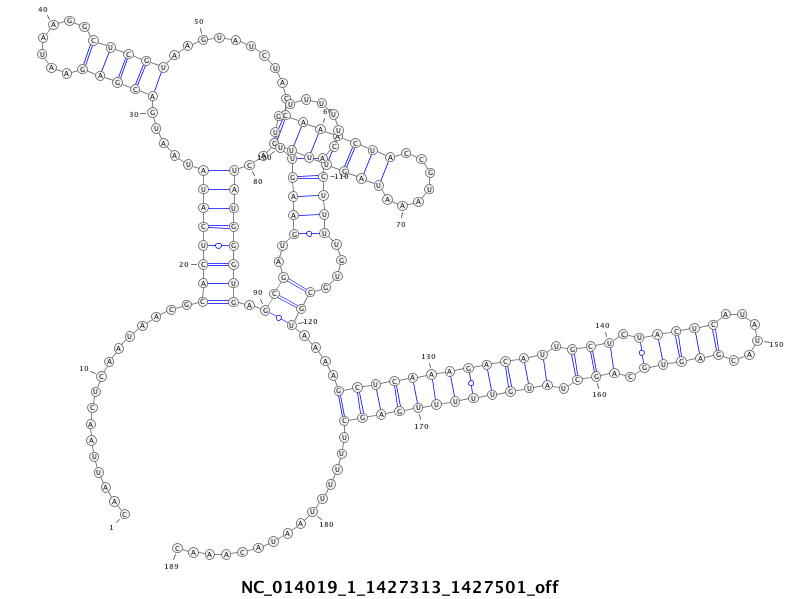
\includegraphics[width=.45\textwidth]{Figures/Ribofinder/NC_014019_1_1427313_1427501_off.png}
    \hfill
    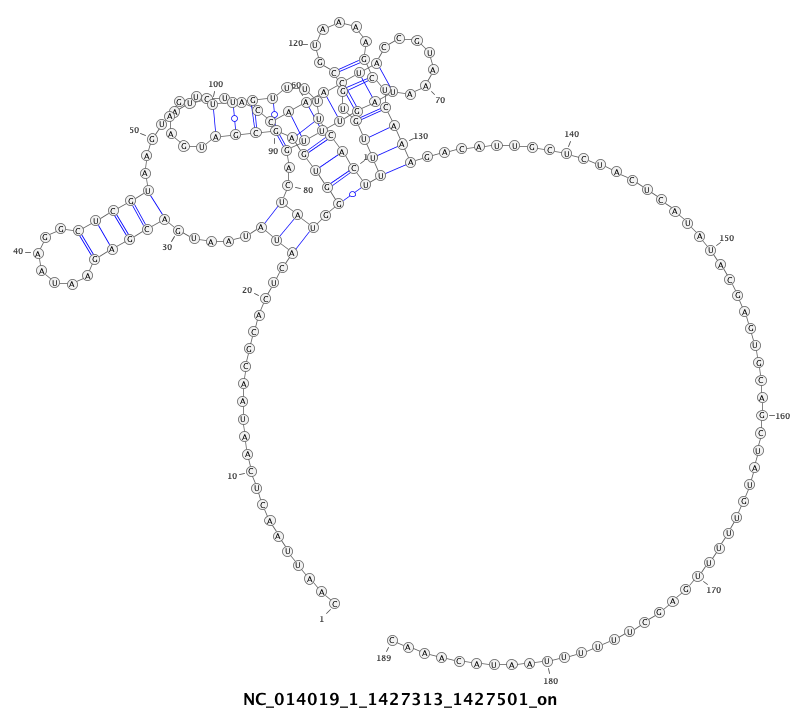
\includegraphics[width=.45\textwidth]{Figures/Ribofinder/NC_014019_1_1427313_1427501_on.png}
    \caption{{\em Left:} the computationally predicted gene-off conformation of sequence NC\_014019.1 1427313-1427501, using \ms{RNAfold} from the ViennaRNA 2.1.8 suite, with dangles disabled and the Turner 1999 energies. This sequence is located upstream of the xpt gene in Bacillus megaterium QM B1551. {\em Right:} the gene-on conformation.}
  \label{fig:example_ss}
\end{figure}

\subsection{Fine-Grained Filtering} \label{sub:fine}

Until now, we have described our approach for generating the 503 guanine \rb candidates in RefSeq, alongside their gene-on and off structures. Unfortunately the experimental validation of all 503 candidates is not tractable, so it was necessary to reduce this collection again to a more manageable size, while only keeping the most promising candidates.

\subsubsection{Using \foldalign to Rank Candidates} \label{ssub:foldalign}
